% Created 2024-07-08 Mon 22:16
% Intended LaTeX compiler: pdflatex
\documentclass[11pt]{article}
\usepackage[utf8]{inputenc}
\usepackage[T1]{fontenc}
\usepackage{ragged2e}
\usepackage{caladea}
\usepackage{graphicx}
\usepackage{longtable}
\usepackage{wrapfig}
\usepackage{rotating}
\usepackage[normalem]{ulem}
\usepackage{amsmath}
\usepackage{amssymb}
\usepackage{capt-of}
\usepackage{hyperref}
\usepackage{fancyhdr}
\title{Novena à Santa Bibiana}
 % \hypersetup{
 %  pdfauthor={},
 %  pdftitle={Novena a/à SANTO_NOME},
 %  pdfkeywords={},
 %  pdfsubject={},
 %  pdfcreator={Emacs 29.4 (Org mode 9.6.15)}, 
 %  pdflang={English}
 % }


\title{
 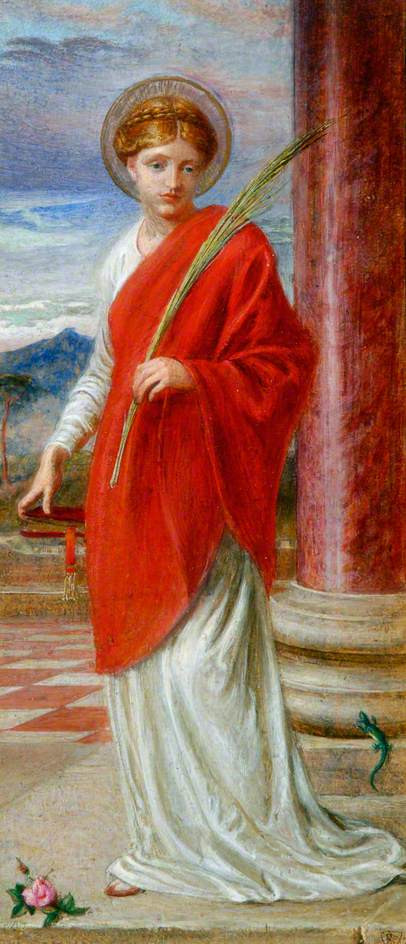
\includegraphics[trim={0 0 0 5cm} , scale=0.3]{./assets/imagem.jpg} \par
  NOVENA À SANTA BIBIANA
}
\author{Garamog, Nina Freitas}
\date{Início da Novena: 23/11 - Data Litúrgica: 02/12}

\begin{document}


\maketitle

\pagestyle{fancy}
  
\centering


% configuração do sumário
\renewcommand{\contentsname}{Sumário}
\tableofcontents

\newpage

\section{História}

\begin{justify}

 Pouco se sabe sobre a vida de santa Bibiana, mas seu nome está registrado no Liber Pontificalis ou Livro dos Pontífices, onde consta que o papa são Simplício (século V) ordenou a construção de uma basílica dedicada a ela em Roma, onde suas relíquias repousam até hoje.

Santa Bibiana nasceu por volta do ano 347 no ambiente sereno de uma família cristã. Seus pais eram Flaviano, prefeito de Roma, e Dafrosa, uma mulher pertencente à nobreza romana. Bibiana tinha uma irmã chamada Demétria.


Com a ascensão de Juliano II ao poder em 361, Flaviano, pai de Bibiana e fervoroso cristão, foi deposto de seu cargo e Aproniano, um pagão muito próximo do novo imperador, foi nomeado em seu lugar.

O prefeito, forçado a retirar-se da vida pública, dedicou-se então a cuidar dos necessitados e perseguidos, além de garantir que os cristãos sacrificados no martírio pudessem sempre ter um enterro digno, de acordo com o mandato da caridade cristã.

Assim que Aproniano soube dessa tarefa assumida por seu antecessor, mandou matá-lo.

Após a morte de Flaviano, Dafrosa e suas duas filhas se desfizeram de seus bens e foram viver na clandestinidade. As três ficaram escondidas, dedicadas à oração constante e vivendo com modéstia. Os tempos eram ruins e tinham que estar preparadas para enfrentar o que viesse.

Apesar do esforço para permanecerem escondidas, as mulheres foram encontradas e obrigadas a renunciar à fé em Cristo. Como se recusaram a fazê-lo, Aproniano executou Dafrosa primeiro, que foi decapitada em 6 de janeiro de 362.

Depois, o prefeito fez uma nova tentativa de forçar Bibiana e Demétria à apostasia. Ele as trancou em uma cela sem nenhuma comida. Demétria morreu de fome antes que pudesse ser submetida a outra provação.

Bibiana foi levada à presença de Aproniano que, para enfraquecer sua vontade, mandou-a para um prostíbulo para ser prostituída. O plano fracassou, pois nenhum homem conseguiu tocá-la. Aproniano ordenou, então, que Bibiana fosse atada a uma coluna e flagelada até a morte.  

Cheia de chagas por todo o corpo, Bibiana entregou sua alma a Deus no altar do martírio, por amor à fé. Embora os soldados tenham jogado seu corpo aos cães, um grupo de cristãos o resgatou e o sepultou junto aos túmulos de seus pais e de sua irmã, bem perto da casa onde ela havia morado.

Pouco tempo depois, quando terminou a perseguição, os cristãos fizeram do lugar um local de culto, onde iam rezar. Décadas depois, o papa Simplício ordenou a construção in situ da atual basílica dedicada à santa, que fica no Monte Esquilino.

\end{justify}
Créditos: \href{https://www.acidigital.com/noticia/53880/hoje-e-celebrada-santa-bibiana-padroeira-dos-que-sofrem-de-epilepsia-e-dores-fortes}{ACI Digital}
\section{Orações}
\subsection{Oração Inicial}

Ó Santa Catarina Labouré, que na Sexta Feira da Paixão entrastes em uma casa e encontrastes cinco mil homens bravos como leões, e com vossa santa palavra, abrandastes o coração de todos. Abrandai o coração de meus inimigos. Se tiverem olhos que não me enxerguem, se tiverem ouvidos que não me escutem, se tiverem pernas que não me sigam, se tiverem mãos que não me toquem. Vós que ouvistes dos lábios da Virgem Imaculada que o perigo será grande, tudo parecerá perdido, mas que ela estará convosco, alcançai-me de Deus, a vossa proteção, e a graça que eu vos peço nessa novena. Amém.

\textbf{(Faça aqui seu pedido)}

\textbf{Pai-Nosso, Ave-Maria, Glória}

\subsection{Oração Final} Imploramos ó Deus a vossa misericórdia pela intercessão da bem-aventurada Santa Catarina Labouré, virgem e religiosa, que vos foi agradável pelo serviço da caridade aos pobres e pela propagação da Medalha Milagrosa de Maria Imaculada Mãe do vosso Filho que convosco vive e reina na unidade do Espírito Santo. Por todos os séculos dos séculos. Amém.

Santa Catarina Labouré, rogai por nós.
\vfill 
Créditos: \href{https://www.youtube.com/watch?v=iuhbMUT5Jsg&list=PLRL6i6PPLb5_yVJcbDOcvhqSL82u_xFHj}{Virtude Plena}
\end{document}
